\documentclass[11pt]{amsart}
\usepackage{a4wide}
\usepackage{amsfonts,amsmath,amssymb,amsthm}
\usepackage{longtable}
\usepackage{listings}
\usepackage{mathptmx} % times font for text and math
\usepackage{xcolor}
% \usepackage{lmodern}
\usepackage{microtype}
\microtypesetup{tracking,kerning,spacing}
\microtypecontext{spacing=nonfrench}

\usepackage[english]{babel}
\usepackage{tikz}

\usepackage[colorlinks,linkcolor=links,citecolor=cites]{hyperref}
\definecolor{links}{rgb}{.2,.1,.5}
\definecolor{cites}{rgb}{.5,.1,.2}

\newcommand\NN{{\mathbb N}}
\newcommand\QQ{{\mathbb Q}}
\newcommand\RR{{\mathbb R}}
\newcommand\ZZ{{\mathbb Z}}

\renewcommand\AA{{\mathsf A}}
\newcommand\BB{{\mathsf B}}
\newcommand\CC{{\mathsf C}}
\newcommand\DD{{\mathsf D}}
\newcommand\EE{{\mathsf E}}
\newcommand\FF{{\mathsf F}}
\newcommand\HH{{\mathsf H}}

\newcommand{\MM}{\mathsf{M}}


\DeclareMathOperator\conv{conv}
\DeclareMathOperator\aff{aff}
\DeclareMathOperator\pos{pos}
\DeclareMathOperator\lin{lin}
\DeclareMathOperator\codim{codim}
\DeclareMathOperator\vertices{vert}
\DeclareMathOperator{\MBP}{\mathsf{MBP}}

\newtheorem{theorem}{Theorem}[section]
\newtheorem{proposition}[theorem]{Proposition}
\newtheorem{corollary}[theorem]{Corollary}
\newtheorem{lemma}[theorem]{Lemma}

\theoremstyle{definition}
\newtheorem{definition}[theorem]{Definition}
\newtheorem{remark}[theorem]{Remark}
\newtheorem{observation}[theorem]{Observation}
\newtheorem{example}[theorem]{Example}
\newtheorem{conjecture}[theorem]{Conjecture}
\newtheorem{problem}[theorem]{Problem}
\newtheorem{challenge}[theorem]{Challenge}


\title{Ehrhart polynomials and splits of Coxeter Matroids}
\author{Julian Pfeifle}
\address{Dept. Matem\`atiques, Universitat Polit\`ecnica de Catalunya}
\email{julian.pfeifle@upc.edu}

\begin{document}

\maketitle

\section{Coxeter matroids}

Matroids are a combinatorial structure that generalizes, for instance,
the concept of families of subspaces of a vector space. One way among
many to associate a matroid~$\MM$ to a configuration~$X$ of
$n$~vectors in a vector space~$V$ is to specify all subsets~$B$ of
$[n]=\{1,2,\dots,n\}$ that index bases of~$V$ among~$X$. Abstractly, a
matroid on~$[n]$ can be characterized as a system~$\MM$ of subsets
of~$[n]$ that satisfies \emph{Steinitz' basis exchange axiom}:

\begin{quote}
  If $A\ne B\in\MM$ and $a\in A\setminus B$, there exists some $b\in B\setminus A$ such that $A-a+b\in\MM$.
\end{quote}

One way to recover geometry from this combinatorial abstraction is to
work with \emph{characteristic vectors}, by assigning to each
basis~$B$ the $0/1$-vector $\chi(B)$ of length~$n$ that has a `1'
precisely in the coordinates indexed by~$B$. The convex hull
\[
  \MBP(\MM) \ = \ \conv\{\chi(B):B\in\MM\}
\]
of these points is called the \emph{matroid base polytope} of~$\MM$.

\medskip Obviously, one can study the polytope of characteristic
vectors associated to any set system, but it is less than clear what,
if anything, one might learn from it. However, in the case of matroids
these polytopes are quite well-behaved:

\begin{itemize}
\item Since all bases have the same cardinality, all characteristic
  vectors $\chi(B)$ lie on a sphere of radius~$\sqrt{|B|}$, and
  therefore all of them are vertices of~$\MBP(\MM)$.

\item Edges reflect basis exchange: Two vertices $\chi(A)$, $\chi(B)$
  span an edge in~$\MBP(\MM)$ iff $A$,~$B$ satisfy Steinitz' axiom.
\end{itemize}

Hidden just beneath the surface of Steinitz' axiom we find the action
of the \emph{symmetric group}~$S_n$ on~$[n]$: we can regard a Steinitz
interchange $a\leftrightarrow b$ as the transposition $(a,b)$, and
such transpositions generate~$S_n$. Geometrically, each edge
of~$\MBP(\MM)$ materializes the orthogonal reflection of its vertices
across a hyperplane of equation $x_i=x_j$, say, and all of
\emph{those} form a very classical object: the hyperplane arrangement
associated to the root system~$\mathsf{A}_{n-1}$.

\medskip There are various more or less abstract definitions to
generalize these concepts from $\mathsf{A}_{n-1}$ and its associated
regular polytope (the simplex) to the other classical root systems:
$\mathsf{BC}_n$ (cubes), $\mathsf{D}_n$, $\mathsf{H}_3$
(dodeca/icosahedron), $\mathsf{H}_4$ (120-cell and 600-cell), $\mathsf{F}_4$
(24-cell), $\mathsf{E}_6$, $\mathsf{E}_7$, $\mathsf{E}_8$, but the
hands-down winner is the following charming theorem by Israel Gelfand
and Vera Serganova:

\medskip
\noindent  \textbf{Theorem-Definition} (Gelfand--Serganova, 1987; cf.~\cite{bgw-2003})

Let $Q$ be a convex polytope. Consider, for each edge $e$ of $Q$, the
hyperplane~$H_e$ orthogonal to~$e$ that passes through its
midpoint. Let $W$~be the group generated by the reflections in
all~$H_e$. Then $W$~is finite iff $Q$~is a Coxeter matroid (polytope).

\begin{figure}[htbp]
  \centering
  \includegraphics[height=4.5cm]{img/cm-polytopes}
\caption{An illustration in~\cite{bgw-2003} of two $\mathsf{BC}_3$ Coxeter matroid polytopes}
\end{figure}

%Even though there's already a textbook \cite{bgw-2003} on the subject,
%in truth we know very little about Coxeter matroid polytopes:

\section{Uniform Coxeter matroids and the Wythoff construction}

The set of bases of the \emph{uniform matroid} $U(k,n)$ is the entire set $\binom{[n]}{k}$, so that the corresponding matroid base polytope is the hypersimplex~$\Delta(k,n)$.
For fixed~$n$, this hypersimplex may be generated by reflecting the point $(1,\dots,1,0,\dots,0)$ with $k$~entries equal to~$1$ in all the hyperplanes $H_{i,j}=\{x\in\RR^n:x_i=x_j\}$, $i<j$, of the fixed root system~$\mathsf{A}_{n-1}$.
The matroid base polytope of any matroid of rank~$k$ on $n$~elements is then a subpolytope of~$\Delta(k,n)$.

Similarly, suppose that $\tau$ is a classical root system of rank~$n$, with some numbering\footnote{For example, you could use the convention in \url{https://en.wikipedia.org/wiki/Root\_system\#Explicit\_construction\_of\_the\_irreducible\_root\_systems}} of its $n$~simple roots.
For any subset $R\subseteq[n]$, the \emph{uniform Coxeter matroid polytope $M_{\tau,R}$ of type~$\tau$ and rings~$R$} is the convex hull of the orbit of a point \emph{not} on the hyperplanes with normal vectors among the simple roots indexed by~$R$, and \emph{on} the hyperplanes with normal vectors \emph{not} indexed by~$R$.
This is called the \emph{Wythoff construction}, and it is traditional to represent~$R$ by drawing rings around the dots corresponding to the hyperplanes indexed by~$R$ in a Coxeter diagram of~$\tau$.
Thus, $\Delta(k,n) = M_{\mathsf{A}_{n-1}, R}$ for any $R\in\binom{[n]}{k}$, but for other root systems distinct choices of~$R$ generally yield distinct uniform Coxeter matroid polytopes.

\begin{example}
  Figure~\ref{fig:b2_0_1} shows the $8$ classes of Coxeter matroids of type $\BB_2$ with $R=\{0,1\}$.
  Figures~\ref{fig:d3_0_1},~\ref{fig:d3_1_2} and~\ref{fig:d3_0_1_2} show the classes of Coxeter matroids of type $\DD_3$ with $R=\{0,1\}$, $R=\{1,2\}$ and $R=\{0,1,2\}$, respectively.
\end{example}

  \begin{figure}[htbp]
    \centering

    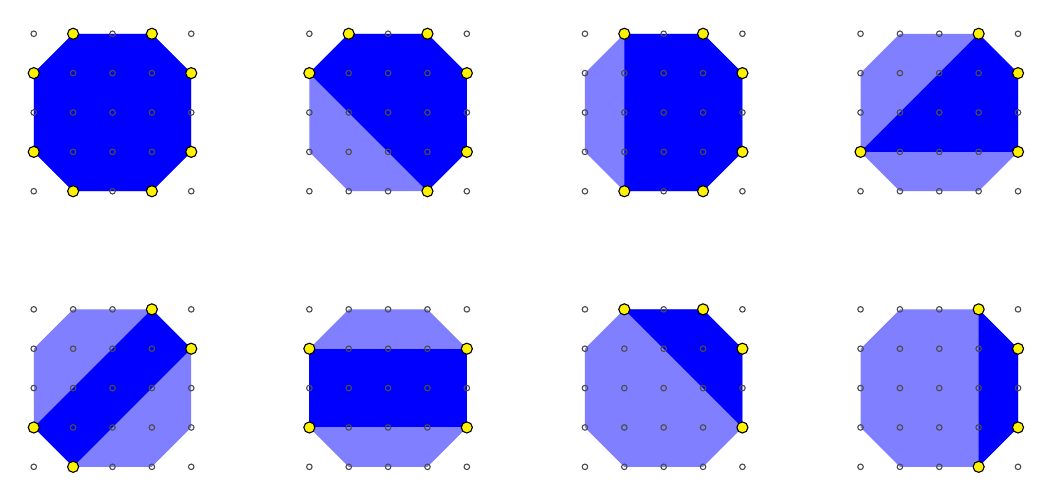
\begin{tikzpicture}[scale=.5]
      \foreach \a/\b/\s in {
        % eight classes of polygons
        % the weird order is because of how wythoff chooses coordinates
        % leave out the initial point 0 from the list
        0/7/{1,4,5,7,6,3,2},
        7/7/{1,4,5,3,2},
        14/7/{1,4,6,3,2},
        21/7/{1,7,2},
        0/0/{1,7,6},
        7/0/{5,7,2},
        14/0/{1,4,2},
        21/0/{1,3,2}%
      } {
        \begin{scope}[shift={(\a,\b)}]

          % label vertices of 8-gon
          \foreach \i/\x/\y in {
            0/2/1, 1/1/2, 2/2/-1, 3/1/-2, 4/-1/2, 5/-2/1, 6/-1/-2, 7/-2/-1
          } {
            \coordinate (pt-\i) at (\x,\y);
          }

          % fill the 8-gon
          \fill [opacity=0.5, blue]
            (pt-0) \foreach \i in {1,4,5,7,6,3,2}{ -- (pt-\i) } -- cycle; 

          % then the representative
          \fill [blue]
            (pt-0) \foreach \i in \s { -- (pt-\i) } -- cycle;

          % draw the grid            
          \foreach \x in {-2,...,2} {
            \foreach \y in {-2,...,2} {
              \draw [black!70] (\x,\y) circle(2pt); 
            }
          }

          % mark the vertices of the representative
          \draw [fill=yellow] (pt-0) circle [radius=4pt];
          \foreach \i in \s {
            \draw [fill=yellow, opacity=1] (pt-\i) circle [radius=4pt];
          }
            
          \end{scope}
      };
    \end{tikzpicture}
    \caption{The $8$ isomorphism classes of Coxeter matroids of type~$\BB_2$ with $R=\{0,1\}$}
    \label{fig:b2_0_1}
  \end{figure}

\begin{figure}[htbp]
  \centering
  \begin{tabular}{cccc}
    \input{img/d3/d3.0_1.0.tikz}
    & 
    \input{img/d3/d3.0_1.1.tikz}
    & 
    \input{img/d3/d3.0_1.2.tikz}
    & 
    \input{img/d3/d3.0_1.3.tikz}
    \\
    \input{img/d3/d3.0_1.4.tikz}
    & 
    % polymake for julian
% Thu Jul  5 11:56:52 2018
% q

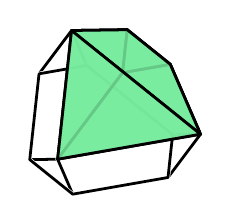
\begin{tikzpicture}[x  = {(0.958794905281451cm,0.110833304484295cm)},
                    y  = {(-0.133135299248327cm,0.988687639709026cm)},
                    z  = {(0.250972750912112cm,0.101058051157179cm)},
                    scale = .5,
                    color = {lightgray}]


  % DEF POINTS
  \coordinate (v0_q) at (2, 1, -1);
  \coordinate (v1_q) at (1, 2, -1);
  \coordinate (v2_q) at (2, -1, 1);
  \coordinate (v3_q) at (1, -1, 2);
  \coordinate (v4_q) at (1, 1, -2);
  \coordinate (v5_q) at (-1, 2, 1);
  \coordinate (v6_q) at (-1, 1, 2);
  \coordinate (v7_q) at (1, -2, 1);
  \coordinate (v8_q) at (-1, -1, -2);
  \coordinate (v9_q) at (-1, -2, -1);
  \coordinate (v10_q) at (-2, 1, 1);
  \coordinate (v11_q) at (-2, -1, -1);


  % EDGES STYLE
  \definecolor{edgecolor_q}{rgb}{ 0,0,0 }
  \tikzstyle{facestyle_q} = [fill=none, fill opacity=0.85, preaction={draw=white, line cap=round, line width=1.5 pt}, draw=edgecolor_q, line width=1 pt, line cap=round, line join=round]


  % FACES and EDGES and POINTS in the right order
  \draw[facestyle_q] (v8_q) -- (v9_q) -- (v11_q) -- (v8_q) -- cycle;
  \draw[facestyle_q] (v4_q) -- (v8_q) -- (v11_q) -- (v10_q) -- (v5_q) -- (v1_q) -- (v4_q) -- cycle;
  \draw[facestyle_q] (v0_q) -- (v2_q) -- (v7_q) -- (v9_q) -- (v8_q) -- (v4_q) -- (v0_q) -- cycle;


  %POINTS


  %FACETS
  \draw[facestyle_q] (v0_q) -- (v4_q) -- (v1_q) -- (v0_q) -- cycle;


  %POINTS


  %FACETS
  \draw[facestyle_q] (v3_q) -- (v2_q) -- (v0_q) -- (v1_q) -- (v5_q) -- (v6_q) -- (v3_q) -- cycle;


  %POINTS


  %FACETS
  \draw[facestyle_q] (v7_q) -- (v2_q) -- (v3_q) -- (v7_q) -- cycle;


  %POINTS


  %FACETS
  \draw[facestyle_q] (v10_q) -- (v6_q) -- (v5_q) -- (v10_q) -- cycle;


  %POINTS


  %FACETS
  \draw[facestyle_q] (v9_q) -- (v7_q) -- (v3_q) -- (v6_q) -- (v10_q) -- (v11_q) -- (v9_q) -- cycle;


  %POINTS


  %FACETS

  % DEF POINTS
  \coordinate (v0_unnamed__1) at (2, 1, -1);
  \coordinate (v1_unnamed__1) at (1, 2, -1);
  \coordinate (v2_unnamed__1) at (2, -1, 1);
  \coordinate (v3_unnamed__1) at (1, 1, -2);
  \coordinate (v4_unnamed__1) at (-1, 2, 1);
  \coordinate (v5_unnamed__1) at (-1, -1, -2);


  % EDGES STYLE
  \definecolor{edgecolor_unnamed__1}{rgb}{ 0,0,0 }

  % FACES STYLE
  \definecolor{facetcolor_unnamed__1}{rgb}{ 0.4667,0.9255,0.6196 }

  \tikzstyle{facestyle_unnamed__1} = [fill=facetcolor_unnamed__1, fill opacity=0.85, draw=edgecolor_unnamed__1, line width=1 pt, line cap=round, line join=round]


  % FACES and EDGES and POINTS in the right order
  \draw[facestyle_unnamed__1] (v3_unnamed__1) -- (v5_unnamed__1) -- (v4_unnamed__1) -- (v1_unnamed__1) -- (v3_unnamed__1) -- cycle;
  \draw[facestyle_unnamed__1] (v2_unnamed__1) -- (v5_unnamed__1) -- (v3_unnamed__1) -- (v0_unnamed__1) -- (v2_unnamed__1) -- cycle;
  \draw[facestyle_unnamed__1] (v0_unnamed__1) -- (v3_unnamed__1) -- (v1_unnamed__1) -- (v0_unnamed__1) -- cycle;


  %POINTS


  %FACETS
  \draw[facestyle_unnamed__1] (v2_unnamed__1) -- (v0_unnamed__1) -- (v1_unnamed__1) -- (v4_unnamed__1) -- (v2_unnamed__1) -- cycle;


  %POINTS


  %FACETS
  \draw[facestyle_unnamed__1] (v4_unnamed__1) -- (v5_unnamed__1) -- (v2_unnamed__1) -- (v4_unnamed__1) -- cycle;


  %POINTS


  %FACETS

\end{tikzpicture}

    & 
    \input{img/d3/d3.0_1.6.tikz}
    & 
  \end{tabular}
  \caption{The $7$ classes of Coxeter matroids of type $\DD_3$ with set of rings $R=\{0,1\}$}
  \label{fig:d3_0_1}
  % These were generated in polymake using the commands
  % $q=wythoff("d3",[0,1],lattice=>1);
  % $r=new Array<Set>(load_data("D3.0_1.cm"));
  % foreach(0..6) {
  %   my $p=new Polytope(VERTICES=>$q->VERTICES->minor($r->[$_],All));  
  %   tikz(compose($q->VISUAL(VertexStyle=>"hidden", FacetStyle=>"hidden"),$p->VISUAL(VertexStyle=>"hidden")),File=>"d3.0_1.$_.tikz");
  % }

\end{figure}

\begin{figure}[htbp]
  \centering
  \begin{tabular}{cccc}
    \input{img/d3/d3.1_2.0.tikz}
    & 
    % polymake for julian
% Thu Jul  5 12:01:37 2018
% q

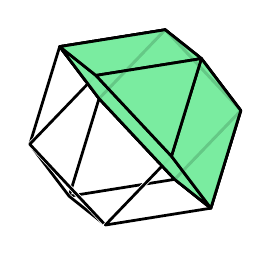
\begin{tikzpicture}[x  = {(0.9cm,-0.076cm)},
                    y  = {(-0.06cm,0.95cm)},
                    z  = {(-0.44cm,-0.29cm)},
                    scale = 1,
                    color = {lightgray}]


  % DEF POINTS
  \coordinate (v0_q) at (1, 1, 0);
  \coordinate (v1_q) at (1, 0, 1);
  \coordinate (v2_q) at (1, 0, -1);
  \coordinate (v3_q) at (0, 1, 1);
  \coordinate (v4_q) at (1, -1, 0);
  \coordinate (v5_q) at (0, 1, -1);
  \coordinate (v6_q) at (0, -1, -1);
  \coordinate (v7_q) at (-1, 1, 0);
  \coordinate (v8_q) at (0, -1, 1);
  \coordinate (v9_q) at (-1, 0, -1);
  \coordinate (v10_q) at (-1, 0, 1);
  \coordinate (v11_q) at (-1, -1, 0);


  % EDGES STYLE
  \definecolor{edgecolor_q}{rgb}{ 0,0,0 }
  \tikzstyle{facestyle_q} = [fill=none, fill opacity=0.85, preaction={draw=white, line cap=round, line width=1.5 pt}, draw=edgecolor_q, line width=1 pt, line cap=round, line join=round]


  % FACES and EDGES and POINTS in the right order
  \draw[facestyle_q] (v2_q) -- (v5_q) -- (v0_q) -- (v2_q) -- cycle;
  \draw[facestyle_q] (v11_q) -- (v6_q) -- (v4_q) -- (v8_q) -- (v11_q) -- cycle;
  \draw[facestyle_q] (v7_q) -- (v9_q) -- (v11_q) -- (v10_q) -- (v7_q) -- cycle;
  \draw[facestyle_q] (v6_q) -- (v2_q) -- (v4_q) -- (v6_q) -- cycle;
  \draw[facestyle_q] (v6_q) -- (v9_q) -- (v5_q) -- (v2_q) -- (v6_q) -- cycle;
  \draw[facestyle_q] (v5_q) -- (v9_q) -- (v7_q) -- (v5_q) -- cycle;
  \draw[facestyle_q] (v11_q) -- (v9_q) -- (v6_q) -- (v11_q) -- cycle;


  %POINTS


  %FACETS
  \draw[facestyle_q] (v10_q) -- (v11_q) -- (v8_q) -- (v10_q) -- cycle;


  %POINTS


  %FACETS
  \draw[facestyle_q] (v7_q) -- (v3_q) -- (v0_q) -- (v5_q) -- (v7_q) -- cycle;


  %POINTS


  %FACETS
  \draw[facestyle_q] (v2_q) -- (v0_q) -- (v1_q) -- (v4_q) -- (v2_q) -- cycle;


  %POINTS


  %FACETS
  \draw[facestyle_q] (v7_q) -- (v10_q) -- (v3_q) -- (v7_q) -- cycle;


  %POINTS


  %FACETS
  \draw[facestyle_q] (v10_q) -- (v8_q) -- (v1_q) -- (v3_q) -- (v10_q) -- cycle;


  %POINTS


  %FACETS
  \draw[facestyle_q] (v8_q) -- (v4_q) -- (v1_q) -- (v8_q) -- cycle;


  %POINTS


  %FACETS
  \draw[facestyle_q] (v3_q) -- (v1_q) -- (v0_q) -- (v3_q) -- cycle;


  %POINTS


  %FACETS

  % DEF POINTS
  \coordinate (v0_unnamed__1) at (1, 1, 0);
  \coordinate (v1_unnamed__1) at (1, 0, 1);
  \coordinate (v2_unnamed__1) at (1, 0, -1);
  \coordinate (v3_unnamed__1) at (0, 1, 1);
  \coordinate (v4_unnamed__1) at (1, -1, 0);
  \coordinate (v5_unnamed__1) at (0, 1, -1);
  \coordinate (v6_unnamed__1) at (0, -1, -1);
  \coordinate (v7_unnamed__1) at (-1, 1, 0);
  \coordinate (v8_unnamed__1) at (-1, 0, -1);


  % EDGES STYLE
  \definecolor{edgecolor_unnamed__1}{rgb}{ 0,0,0 }

  % FACES STYLE
  \definecolor{facetcolor_unnamed__1}{rgb}{ 0.4667,0.9255,0.6196 }

  \tikzstyle{facestyle_unnamed__1} = [fill=facetcolor_unnamed__1, fill opacity=0.85, draw=edgecolor_unnamed__1, line width=1 pt, line cap=round, line join=round]


  % FACES and EDGES and POINTS in the right order
  \draw[facestyle_unnamed__1] (v5_unnamed__1) -- (v0_unnamed__1) -- (v2_unnamed__1) -- (v5_unnamed__1) -- cycle;
  \draw[facestyle_unnamed__1] (v4_unnamed__1) -- (v6_unnamed__1) -- (v2_unnamed__1) -- (v4_unnamed__1) -- cycle;
  \draw[facestyle_unnamed__1] (v5_unnamed__1) -- (v2_unnamed__1) -- (v6_unnamed__1) -- (v8_unnamed__1) -- (v5_unnamed__1) -- cycle;
  \draw[facestyle_unnamed__1] (v7_unnamed__1) -- (v5_unnamed__1) -- (v8_unnamed__1) -- (v7_unnamed__1) -- cycle;
  \draw[facestyle_unnamed__1] (v3_unnamed__1) -- (v7_unnamed__1) -- (v8_unnamed__1) -- (v6_unnamed__1) -- (v4_unnamed__1) -- (v1_unnamed__1) -- (v3_unnamed__1) -- cycle;


  %POINTS


  %FACETS
  \draw[facestyle_unnamed__1] (v3_unnamed__1) -- (v0_unnamed__1) -- (v5_unnamed__1) -- (v7_unnamed__1) -- (v3_unnamed__1) -- cycle;


  %POINTS


  %FACETS
  \draw[facestyle_unnamed__1] (v2_unnamed__1) -- (v0_unnamed__1) -- (v1_unnamed__1) -- (v4_unnamed__1) -- (v2_unnamed__1) -- cycle;


  %POINTS


  %FACETS
  \draw[facestyle_unnamed__1] (v3_unnamed__1) -- (v1_unnamed__1) -- (v0_unnamed__1) -- (v3_unnamed__1) -- cycle;


  %POINTS


  %FACETS

\end{tikzpicture}

    & 
    \input{img/d3/d3.1_2.2.tikz}
    & 
    \input{img/d3/d3.1_2.3.tikz}
    \\
    \input{img/d3/d3.1_2.4.tikz}
    & 
    \input{img/d3/d3.1_2.5.tikz}
  \end{tabular}
  \caption{The $6$ classes of Coxeter matroids of type $\DD_3$ with set of rings $R=\{1,2\}$}
  \label{fig:d3_1_2}
\end{figure}

\begin{figure}[htbp]
  \centering
  \begin{tabular}{cccccc}
    \input{img/d3/d3.0_1_2.0.tikz}
    & 
      \input{img/d3/d3.0_1_2.1.tikz}
    & 
      \input{img/d3/d3.0_1_2.2.tikz}
    & 
      \input{img/d3/d3.0_1_2.3.tikz}
    &
    \input{img/d3/d3.0_1_2.4.tikz}
    & 
    \input{img/d3/d3.0_1_2.5.tikz}
    \\ 
    \input{img/d3/d3.0_1_2.6.tikz}
    & 
      \input{img/d3/d3.0_1_2.7.tikz}
    & 
      \input{img/d3/d3.0_1_2.8.tikz}
    & 
      \input{img/d3/d3.0_1_2.9.tikz}
    &
    \input{img/d3/d3.0_1_2.10.tikz}
    & 
    \input{img/d3/d3.0_1_2.11.tikz}
    \\ 
    \input{img/d3/d3.0_1_2.12.tikz}
    & 
      \input{img/d3/d3.0_1_2.13.tikz}
    & 
      \input{img/d3/d3.0_1_2.14.tikz}
    & 
      \input{img/d3/d3.0_1_2.15.tikz}
    &
    \input{img/d3/d3.0_1_2.16.tikz}
    & 
    \input{img/d3/d3.0_1_2.17.tikz}
    \\ 
    \input{img/d3/d3.0_1_2.18.tikz}
    & 
      \input{img/d3/d3.0_1_2.19.tikz}
    & 
      % polymake for julian
% Thu Jul  5 12:06:49 2018
% q

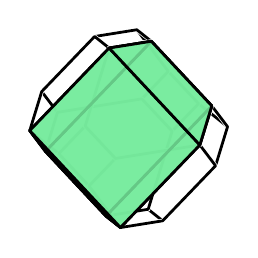
\begin{tikzpicture}[x  = {(0.9cm,-0.076cm)},
                    y  = {(-0.06cm,0.95cm)},
                    z  = {(-0.44cm,-0.29cm)},
                    scale = .4,
                    color = {lightgray}]


  % DEF POINTS
  \coordinate (v0_q) at (3, 1, 0);
  \coordinate (v1_q) at (1, 3, 0);
  \coordinate (v2_q) at (3, 0, 1);
  \coordinate (v3_q) at (3, 0, -1);
  \coordinate (v4_q) at (1, 0, 3);
  \coordinate (v5_q) at (1, 0, -3);
  \coordinate (v6_q) at (0, 3, 1);
  \coordinate (v7_q) at (3, -1, 0);
  \coordinate (v8_q) at (0, 3, -1);
  \coordinate (v9_q) at (0, 1, 3);
  \coordinate (v10_q) at (1, -3, 0);
  \coordinate (v11_q) at (0, 1, -3);
  \coordinate (v12_q) at (0, -1, -3);
  \coordinate (v13_q) at (-1, 3, 0);
  \coordinate (v14_q) at (0, -1, 3);
  \coordinate (v15_q) at (0, -3, -1);
  \coordinate (v16_q) at (-3, 1, 0);
  \coordinate (v17_q) at (0, -3, 1);
  \coordinate (v18_q) at (-1, 0, -3);
  \coordinate (v19_q) at (-1, 0, 3);
  \coordinate (v20_q) at (-3, 0, -1);
  \coordinate (v21_q) at (-3, 0, 1);
  \coordinate (v22_q) at (-1, -3, 0);
  \coordinate (v23_q) at (-3, -1, 0);


  % EDGES STYLE
  \definecolor{edgecolor_q}{rgb}{ 0,0,0 }
  \tikzstyle{facestyle_q} = [fill=none, fill opacity=0.85, preaction={draw=white, line cap=round, line width=1.5 pt}, draw=edgecolor_q, line width=1 pt, line cap=round, line join=round]


  % FACES and EDGES and POINTS in the right order
  \draw[facestyle_q] (v0_q) -- (v3_q) -- (v5_q) -- (v11_q) -- (v8_q) -- (v1_q) -- (v0_q) -- cycle;
  \draw[facestyle_q] (v10_q) -- (v17_q) -- (v22_q) -- (v15_q) -- (v10_q) -- cycle;
  \draw[facestyle_q] (v16_q) -- (v20_q) -- (v23_q) -- (v21_q) -- (v16_q) -- cycle;
  \draw[facestyle_q] (v5_q) -- (v3_q) -- (v7_q) -- (v10_q) -- (v15_q) -- (v12_q) -- (v5_q) -- cycle;
  \draw[facestyle_q] (v11_q) -- (v5_q) -- (v12_q) -- (v18_q) -- (v11_q) -- cycle;


  %POINTS


  %FACETS
  \draw[facestyle_q] (v8_q) -- (v11_q) -- (v18_q) -- (v20_q) -- (v16_q) -- (v13_q) -- (v8_q) -- cycle;


  %POINTS


  %FACETS
  \draw[facestyle_q] (v12_q) -- (v15_q) -- (v22_q) -- (v23_q) -- (v20_q) -- (v18_q) -- (v12_q) -- cycle;


  %POINTS


  %FACETS
  \draw[facestyle_q] (v17_q) -- (v14_q) -- (v19_q) -- (v21_q) -- (v23_q) -- (v22_q) -- (v17_q) -- cycle;


  %POINTS


  %FACETS
  \draw[facestyle_q] (v1_q) -- (v8_q) -- (v13_q) -- (v6_q) -- (v1_q) -- cycle;


  %POINTS


  %FACETS
  \draw[facestyle_q] (v7_q) -- (v3_q) -- (v0_q) -- (v2_q) -- (v7_q) -- cycle;


  %POINTS


  %FACETS
  \draw[facestyle_q] (v9_q) -- (v6_q) -- (v13_q) -- (v16_q) -- (v21_q) -- (v19_q) -- (v9_q) -- cycle;


  %POINTS


  %FACETS
  \draw[facestyle_q] (v4_q) -- (v9_q) -- (v19_q) -- (v14_q) -- (v4_q) -- cycle;


  %POINTS


  %FACETS
  \draw[facestyle_q] (v7_q) -- (v2_q) -- (v4_q) -- (v14_q) -- (v17_q) -- (v10_q) -- (v7_q) -- cycle;


  %POINTS


  %FACETS
  \draw[facestyle_q] (v2_q) -- (v0_q) -- (v1_q) -- (v6_q) -- (v9_q) -- (v4_q) -- (v2_q) -- cycle;


  %POINTS


  %FACETS

  % DEF POINTS
  \coordinate (v0_unnamed__1) at (3, 1, 0);
  \coordinate (v1_unnamed__1) at (1, 3, 0);
  \coordinate (v2_unnamed__1) at (3, 0, 1);
  \coordinate (v3_unnamed__1) at (0, 3, 1);
  \coordinate (v4_unnamed__1) at (0, -3, 1);
  \coordinate (v5_unnamed__1) at (-3, 0, 1);
  \coordinate (v6_unnamed__1) at (-1, -3, 0);
  \coordinate (v7_unnamed__1) at (-3, -1, 0);


  % EDGES STYLE
  \definecolor{edgecolor_unnamed__1}{rgb}{ 0,0,0 }

  % FACES STYLE
  \definecolor{facetcolor_unnamed__1}{rgb}{ 0.4667,0.9255,0.6196 }

  \tikzstyle{facestyle_unnamed__1} = [fill=facetcolor_unnamed__1, fill opacity=0.85, draw=edgecolor_unnamed__1, line width=1 pt, line cap=round, line join=round]


  % FACES and EDGES and POINTS in the right order
  \draw[facestyle_unnamed__1] (v0_unnamed__1) -- (v2_unnamed__1) -- (v4_unnamed__1) -- (v6_unnamed__1) -- (v0_unnamed__1) -- cycle;
  \draw[facestyle_unnamed__1] (v0_unnamed__1) -- (v6_unnamed__1) -- (v7_unnamed__1) -- (v1_unnamed__1) -- (v0_unnamed__1) -- cycle;
  \draw[facestyle_unnamed__1] (v5_unnamed__1) -- (v3_unnamed__1) -- (v1_unnamed__1) -- (v7_unnamed__1) -- (v5_unnamed__1) -- cycle;
  \draw[facestyle_unnamed__1] (v6_unnamed__1) -- (v4_unnamed__1) -- (v5_unnamed__1) -- (v7_unnamed__1) -- (v6_unnamed__1) -- cycle;


  %POINTS


  %FACETS
  \draw[facestyle_unnamed__1] (v4_unnamed__1) -- (v2_unnamed__1) -- (v3_unnamed__1) -- (v5_unnamed__1) -- (v4_unnamed__1) -- cycle;


  %POINTS


  %FACETS
  \draw[facestyle_unnamed__1] (v3_unnamed__1) -- (v2_unnamed__1) -- (v0_unnamed__1) -- (v1_unnamed__1) -- (v3_unnamed__1) -- cycle;


  %POINTS


  %FACETS

\end{tikzpicture}

    & 
      \input{img/d3/d3.0_1_2.21.tikz}
  \end{tabular}
  \caption{The $22$ classes of Coxeter matroids of type $\DD_3$ with set of rings $R=\{0,1,2\}$}
  \label{fig:d3_0_1_2}
\end{figure}

\section{Challenges}

\subsection{Enumeration}

Complete enumeration of all matroids or Coxeter matroids doesn't make much sense, given the large symmetry groups that operate on these objects.
Therefore, we will always enumerate only pairwise non-isomorphic Coxeter matroids, where we consider two Coxeter matroid polytopes $M_{\tau,R}$, $M'_{\tau.R}$ to be isomorphic if they are related by a symmetry induced by the root system~$\tau$. 

The number of isomorphism classes of $\AA_{n-1}$-matroids of rank~$r$ on $n$~elements is known for $r \le 3$ and $n \le 12$,
for $r=4$ and $n \le 10$,
and for $r=5$ and $n \le 9$.
The largest computation among these is that of Matsumoto et al~\cite{bremner-2012}, who determined the number of isomorphism classes for $(r,n)=(4,10)$ to be 4\,886\,380\,924.

Tables~\ref{tab:cm3} and~\ref{tab:cm4} summarize the results of our enumeration isomorphism classes of some Coxeter matroids using \texttt{polymake}~\cite{DMV:polymake}.

\begin{challenge}
  Confirm or correct, and extend if possible, the data in Tables~\ref{tab:cm3} and~\ref{tab:cm4}.
\end{challenge}

\newcommand{\te}[2]{\textbf{#1} \raisebox{-3pt}{\footnotesize \textcolor{black!50}{#2}}} % for table entries in enumeration tables

\begin{table}[htbp]
  \centering
  \renewcommand{\arraystretch}{1.5}
  \begin{tabular}[c]{c|ccccccc}
    Root system $\tau$ $\backslash$ Rings $R$ & $0$ & $1$ & $2$ & $01$ & $02$ & $12$ & $012$ \\\hline
    $\BB_3,\CC_3$ & \te{3}{6} & \te{22}{12} & \te{9}{8} & \te{83}{24} & \te{79}{24} & \te{109}{24} & \te{}{48} \\
    $\DD_3$ & \te{2}{6} & \te{1}{4} & \te{1}{4} & \te{7}{12} & \te{7}{12} & \te{6}{12} & \te{22}{24} \\
    $\HH_3$ & \te{1089}{20} & \te{9701}{30} & \te{57}{12} & \te{}{60} & \te{}{60} & \te{}{60} & \te{}{120}\\\hline
  \end{tabular}

  \medskip
  \caption{In boldface, the known numbers of isomorphism classes of $3$-dimensional Coxeter matroids.
    Smaller, lowered and gray, the number of vertices of the uniform Coxeter matroid~$M_{\tau,R}$ of which the isomorphism classes are subpolytopes.
    Note that the following choices of rings~$R$ yield combinatorially isomorphic uniform Coxeter matroids:
    For $\DD_3$,
    $R\in\{1,2\}$,
    $R\in\{01,02\}$
  }
  \label{tab:cm3}
\end{table}

\begin{table}[htbp]
  \centering
  \renewcommand{\arraystretch}{1.5}
  \begin{tabular}[c]{c|cccccccccc}
    Root system $\tau$ $\backslash$ Rings $R$
    & $0$ & $1$ & $2$ & $3$
    & $01$ & $02$ & $03$
    & $12$ & $13$ & $23$
    \\\hline 
    $\BB_4,\CC_4$ & \te{4}{8} & \te{133}{24} & \te{873}{32} & \te{67}{16} & \te{}{48} & \te{}{96} & \te{}{64} & \te{}{96} & \te{}{96} & \te{}{64} \\
    $\DD_4$ & \te{3}{8} & \te{67}{24} & \te{3}{8} & \te{3}{8} & \te{}{48} & \te{}{32} & \te{}{32} & \te{}{48} & \te{}{48} & \te{}{32} \\
    $\FF_4$ & \te{2345}{24} & \te{}{96} & \te{}{96} & \te{2345}{24} & \te{}{192} & \te{}{288} & \te{}{144} & \te{}{288} & \te{}{288} & \te{}{192}\\
    $\HH_4$ & \te{}{600} & \te{}{1200} & \te{}{720} & \te{}{120} & \te{}{2400} & \te{}{3600} & \te{}{2400} & \te{}{3600} & \te{}{3600} & \te{}{1440} \\\hline
  \end{tabular}

  \medskip
  \caption{In boldface, the known numbers of isomorphism classes of $4$-dimensional Coxeter matroids.
    Smaller, lowered and gray, the number of vertices of the uniform Coxeter matroid~$M_{\tau,R}$ of which the isomorphism classes are subpolytopes.
    Note that the following choices of rings~$R$ yield combinatorially isomorphic uniform Coxeter matroids:
    For $\DD_4$,
    $R\in\{0,2,3\}$,
    $R\in\{01,12,13\}$,
    $R\in\{02,03,23\}$;
    For $\FF_4$,
    $R\in\{0,3\}$,
    $R\in\{1,2\}$;
    etc
  }
  \label{tab:cm4}
\end{table}

\subsection{Facets of Coxeter matroids}

\begin{challenge}
  What can you say about the combinatorial types of faces of Coxeter
  matroid polytopes? For $\mathsf{A}_{n-1}$, the only possible
  $2$-faces are triangles and squares~\cite[Theorem 1.12.8]{bgw-2003},
  but for the other types even this very basic question seems to be
  open (though easy).
\end{challenge}

\begin{challenge}
  Let $\tau$ be a root system of dimension~$d$.
  Describe and count the facets of~$M_{\tau,[d]}$.
\end{challenge}

\begin{challenge}
  Given a subset $F\subset[d]$, is there always a facet of~$M_{\tau,[d]}$ whose edges are parallel to the vectors in~$F$?
\end{challenge}

\begin{challenge}\label{prob:facet-orthogonal-root}
  Classify the facets of $M_{\tau,[d]}$ that are orthogonal to a root vector.
\end{challenge}

\begin{challenge}
  Using the result of Challenge~\ref{prob:facet-orthogonal-root}, determine if there are Coxeter matroids all of whose facets are orthogonal to a root.
\end{challenge}

\begin{challenge}
  Determine the symmetry classes of facets of $M_{\tau,[d]}$ under the action of~$\tau$.
\end{challenge}

\begin{challenge}\label{prob:same-hyperplanes}
  The hyperplanes defining facets of~$M_{\BB_3,02}$ (which are squares, rectangles and triangles)
  are parallel to the hyperplanes defining facets of~$M_{\BB_3,012}$ (which are octagons~---from cutting off the vertices of a square---~,
  hexagons~---from cutting off the vertices of a triangle---~, and rectangles).
  The same appears to happen for~$M_{\DD_3,12}$.

  For which other types does this happen, in general dimension~$d$?
\end{challenge}

\begin{conjecture}
  Let $\tau$ be a root system of dimension~$d$, and let $Q\subset M_{\tau,R}$ be a Coxeter matroid.
  Then each facet of~$Q$ is parallel to a facet of~$M_{\tau,[d]}$.
\end{conjecture}

\begin{challenge}
  Let $\tau$ be a root system of dimension~$d$.
  Describe the orbits of the vectors in~$\tau$ under~$\tau$,
  and thus determine the equivalence classes of edges of Coxeter matroids.
\end{challenge}


\subsection{Concordant Coxeter Matroids}

\begin{definition}
  A Coxeter matroid $Q\subseteq M_{\tau,R}$ is \emph{concordant} if each facet of~$Q$ is parallel to a facet of~$M_{\tau,R}$ (and not just of~$M_{\tau,[d]}$).
\end{definition}

\begin{example}
  Our partial enumeration yields the results depicted in \texttt{concordant-examples.pdf}.
\end{example}

\begin{observation}
  By Challenge~\ref{prob:same-hyperplanes}, all Coxeter matroids belonging to $M_{\BB_3,02}$ or $M_{\DD_3,12}$ are concordant. 
\end{observation}

\begin{definition}
  A \emph{picky} concordant matroid is a concordant matroid all of whose facets belong to the same symmetry type.
\end{definition}

\begin{challenge}
  Which types have picky concordant matroids, and how many of them? This is what we know so far:
  \begin{center}
    \begin{tabular}[c]{c|ccccccccc}
      type $\backslash$ rings& 0 & 1 & 2 & 3 & 01 & 02 & 12 & 012\\\hline
      $\BB_3$     & 1 & 0 & 1 &   & 1  & 1  & 2  \\
      $\DD_3$     & 0 &   &   &   & 0  &    & 0  & 0 \\
      $\BB_4$     & 1 & 0 & 0 & 1\\
      $\DD_4$     & 0 & 0 & 0 & 0\\
      $\FF_4$     & 12
    \end{tabular}
  \end{center}
  Explain this table! Can you extend it to $\BB_n$, $\DD_n$ for $n\ge5$?
\end{challenge}

\subsection{Lattice Coxeter matroids}

The classical root systems are all \emph{crystallographic}, with the exception of $H_3$ and $H_4$.
This means that the root vectors generate a lattice.

\begin{challenge}\label{chall:root-lattice}
  For all crystallographic root systems, find out if there is a canonical realization of each uniform Coxeter matroid as a lattice polytope in the root lattice
\end{challenge}

\begin{challenge}
  If the answer to Challenge~\ref{chall:root-lattice} is positive, find out if there is any relation between the Ehrhart polynomials of the Coxeter matroid polytopes of a fixed uniform Coxeter matroid.
\end{challenge}

\subsection{Splits of Coxeter matroids}

A very important construction in toric and tropical geometry is the
subdivision, in the case $\mathsf{A}_{n-1}$, of matroid polytopes into
smaller matroid polytopes. This was first considered by
Lafforgue~\cite{l-2003}. Speyer~\cite{speyer-2008} conjectured that
the subdivision corresponding to \emph{series-parallel} matroids have
the largest number of faces, and he proved this in the case of
tropical linear spaces.

\begin{challenge}
  What can you say about subdivisions of Coxeter
  matroid polytopes into smaller Coxeter matroid polytopes?
\end{challenge}

\bibliographystyle{plain}
\bibliography{coxeter}

\end{document}
